\section{Mozilla}
\label{sec:mozilla}

\par \href{http://www.mozilla.org/}{Mozilla foundation} is a huge community that involves different types of users and has a central message applied to all its levels:

\par \textit{"Our mission is to promote openness, innovation \& opportunity on the Web."} In \href{http://www.mozilla.org/about/manifesto.html}{Mozilla Manifesto} you can read the whole document about freedom and accessibility that they apply day by day.

\par The Foundation is consolidated by years of dedication to freedom of the web through its flagship Firefox. Since Netscape released the source code in 1998 Mozilla got down to work to develop a web browser from FLOSS source code they received from Netscape.

\par Mozilla wanted a free internet because IExplorer market share was 90\%. Was a private market and now this trend has changed. Source: \href{http://gs.statcounter.com/#browser-ww-yearly-2008-2013}{StatCounter Global Stats - Browser Market Share}

\subsection{Technologies}

\par There is a bunch of technologies surrounding Mozilla development communities and of course, projects:

\begin{itemize}
	\item \textit{Firefox} - Web Browser with a particularity that doesn't have portability to IOS because it uses Gecko instead of Webkit to render content. Apple doesn't allow a browser (or anything) that is not reder using Webkit.
	\item \textit{FirefoxOS} - New Mobile operative system based in HTML5 and Browser Oriented.
	\item \textit{Thunderbird} - eMail management but abandoned project. Developers have changed to Mozilla.
	\item \textit{Camino} - MacOS Mozilla Browser using Webkit
	\item \textit{Seamonkey} - Firefox, Thunderbird, Chat, Web Editor.
	\item \textit{Sundbird/Lightning} - Calendar project from Mozilla.
	\item \textit{XULRunner} - It's like Java Virtual Machine allowing multiplatform products oriented to Mozilla packages.
\end{itemize}

And of course, developer tools to work with Mozilla community:

\begin{itemize}
	\item \textit{Mailing lists}- For developers, information, everything related to \href{https://lists.mozilla.org/listinfo}{Mozilla}.
	\item \textit{Bug Tracking System}-\href{https://bugzilla.mozilla.org/}{Bugzilla}for every product.
	\item \textit{Source Code Management}- Baazar, Mercurial, SVN, CVS.
	\item \textit{MXR}- Cross references about the code from Mozilla (\href{http://mxr.mozilla.org/}{mxr}).
	\item \textit{Forge for scm}- GitHub.
	\item \textit{QMO}-Home of Mozilla's testing and \href{http://quality.mozilla.org/}{quality assurance community}.
	\item \textit{Crash Stats} - \emph{Continuous integration} server output visualizations using \href{https://github.com/mozilla/socorro}{Socorro}.
	\item \textit{Graph CI}- Graphic visualization for every built from the code in\href{http://graphs.mozilla.org/}{graph section}.
	\item \textit{Tinderbox}- Tool to navigate through \href{http://tinderbox.mozilla.org/showbuilds.cgi}{build logs and results}.
\end{itemize}

\subsection{How to contribute}

\par Mozilla community is very community, this statement may sound redundant, but would be an accurate definition. He moved away from the technology and developers as standard for any project.

\begin{figure}[H]
    \centering
    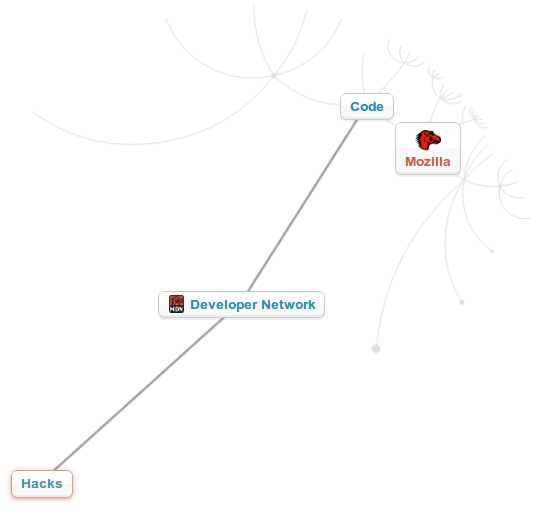
\includegraphics[width=0.7\textwidth]{mozilla-community-developers}
    \caption{}
    \label{community-dev}
\end{figure}

\par Mozilla has the basic steps as other FLOSS projects for \href{http://www.mozilla.org/es-ES/contribute/}{How to Contribute} and gives you an opportunity to contribute in more than one way looking for a chance:

\begin{itemize}
	\item Help for Users
	\item Quality control
	\item Programming
	\item Spread the word
	\item location
	\item Web Development
	\item Accessories
	\item graphic Design
	\item Documentation and drafting
	\item Education
\end{itemize}

\par Furthermore gives you the opportunity to look for contribution near your location, a very useful tool. Mozilla invites you to be part of an Open Web. You don't have to be the smartest guy in the world they do this work spreading that all help is good an they will find for you the best place to help \textit{everyone} with your contribution.

% section mozilla (end)
